% Main paper template (L4DC 2027).  Every result or parameter numeral is a double-brace placeholder resolved from
% results/section_numbers.json by tools/build_main.py; do not type numbers into main.tex.
% Preamble: paper/preamble_jmlr.tex (venue class l4dc2027) verbatim via \input, then local macros in main_macros.tex.
\input{preamble_jmlr}
\input{main_macros}

\title[One Budget for Every Gap]{One Budget for Every Gap: Certifying Reduced-Order, Quantized, Sampled-Data Neural Barrier Controllers on the Full Plant}
\author{\Name{Author One}\Email{author.one@institution.edu}\\ \addr Institution, City, Country}

\begin{document}
\maketitle

\begin{abstract}
A neural safety filter for a high-dimensional plant is verified on a reduced model, in exact arithmetic and continuous time, but runs as a quantized network and a look-up table, sampled and latched, on the full plant under a bounded disturbance. We charge each gap to one term of a single control-authority budget on a reduced control barrier function. The reduced-order tail, the table quantization, the verified deviation of the quantized network, the latch lag, the sample-and-hold error and the adversary each consume part of the certified authority $\delta_{\mathrm{cert}}$. When their sum does not exceed it, and under standing hypotheses on the plant, the reduction and the initial state, the full-order plant is safe for all time. For underdamped second-order port-Hamiltonian plants with uniform modal damping and $m \le K$ actuators, $\delta_{\mathrm{cert}}$ has a closed-form lower bound. A coupled twin-network CROWN pass bounds the deviation of the quantized network from its teacher, and both this bound and a closed-form companion are of order $2^{-b_B}$. On a 320-state reaction--diffusion--advection lattice at P\'eclet 20, open-loop unsafe on every seed, the budget closes at utilisation 0.931 and no certified trajectory leaves the safe set. Without the tail or quantization term, the certificate accepts a controller the plant then violates, and the single-rate alternative is refused at the deployed period. The certified plant filters its advection spectrally, and a sweep over the filter weight maps where the $L^2$-based tail bound is non-vacuous; unfiltered advection is refused. Every constant is computed in double precision from the operators, and the code reproduces every number.
\end{abstract}

\begin{keywords}
control barrier functions; sampled-data control; reduced-order models; neural network verification; quantized neural networks; port-Hamiltonian systems; safety certificates
\end{keywords}

% =====================================================================================================================
\section{Introduction}
\label{sec:intro}

A neural safety filter is rarely verified on the system it runs on. It is designed on a reduced model because the plant is too large. It is specified as a floating-point teacher, although the deployed student is a $b_B$-bit network paired with a $b_A$-bit look-up table. It is analysed in continuous time because that is where barrier conditions are stated, while the hardware samples the state at period $T_s$ and latches two commands after two different delays. It is certified against a nominal model, while the plant is driven by an unknown bounded disturbance. Each of these gaps has its own remedy; what is missing is a statement of what survives all of them at once, on the plant, for all time.

We give one: each of the six gaps is charged to one term of one inequality. When the inequality closes, under standing hypotheses on the plant, the reduction and the initial state, the full-order plant is safe for all time; when the tail or the quantization term is dropped, the certificate accepts a controller the plant then violates. The single-rate alternative, refused at the deployed period, leaves the safe set at a longer one, and so does the plant under an adversary beyond the certified level. Every gap consumes part of the certified control authority $\dcert$ of a reduced barrier, the amount by which the teacher holds the barrier rate above its prescribed decay on a shell near the boundary. The terms are not safety factors stacked on a nominal design; each bounds one summand of the exponentially weighted integral of the reduced barrier rate over one sampling interval along the full-order flow.

On a 320-state telegraph reaction--diffusion--advection lattice at P\'eclet 20, open-loop unsafe on all 16 seeds, the deployed configuration consumes 0.931 of its certified authority and no certified trajectory leaves the safe set. The certified plant filters its advection spectrally, unfiltered advection is refused, and a sweep over the filter weight locates where the certificate stops accepting. The contributions are four. (i) The budget \eqref{eq:budget}, named the Certified Control Authority Condition, and Theorem~\ref{thm:main_cbf}: full-order safety in continuous time, for all time and under a bounded adversary, of a reduced-order, quantized, multi-rate sampled-data neural controller (Sections~\ref{sec:budget} and~\ref{sec:main}). (ii) A closed-form lower bound on $\dcert$ for class-(H) reduced models with uniform modal damping, $\gamma < 2\omega_{\min}$ and $m \le K$ actuators, within one percent of brute force in both regimes (Lemma~\ref{lem:delta_cert_classH}, Table~\ref{tab:budget}). (iii) A bound on the deviation of a quantized GroupSort-2 student from its isometric teacher, obtained by a twin-network CROWN pass, an instance of differential verification, with a closed-form companion; both are of order $2^{-b_B}$ (Proposition~\ref{prop:twin_crown}, Section~\ref{sec:numerics}). (iv) The certificate on a 320-state lattice in two regimes, with ablations, refusals and the frontier sweep (Section~\ref{sec:numerics}, Figure~\ref{fig:results}). Section~\ref{sec:setting} fixes the setting, Section~\ref{sec:budget} derives the six terms, Section~\ref{sec:main} states the theorem, Section~\ref{sec:numerics} certifies the lattice and Section~\ref{sec:limits} states what the certificate does not cover.

\paragraph{Sampled-data barriers.}
Control barrier functions certify forward invariance for continuous-time control-affine systems \citep{ames2017cbf,ames2019theory}. Sampled-data versions tighten the condition to hold between samples, under input delay \citep{singletary2020sampled}, for a fixed time step \citep{breeden2022sampled}, through approximate discrete-time models \citep{taylor2022sampled}, or by a zero-order condition free of derivatives \citep{tan2025zeroorder}. The closest work is \citet{niu2024sampling}, which bounds the gap between digital and true barrier constraints under sampled, quantized state measurements and finite-precision coefficients on the full-order plant; here the quantized object is a learned controller and a reduced-order tail term is added. These works charge neither the tail term nor the verification slack.

\paragraph{Reduced-order and model-error barriers.}
Robust and input-to-state safe barriers add a margin for an unstructured disturbance \citep{jankovic2018robust,kolathaya2019issf}. Reduced-order designs filter on a low-dimensional model and carry a tracking error to the full system \citep{singletary2022kinematic,molnar2022modelfree,cohen2024romsurvey}. The closest reduced-order work is \citet{cohen2025romsynthesis}, which relates the two models by projection maps, bounds their discrepancy by an assumed supremum and proves invariance of a safe set inflated by that bound. Here the residual is computed from the Petrov--Galerkin truncation of a dissipative port-Hamiltonian operator and enters as one budget term; these works charge no quantization, slack, lag or hold term.

\paragraph{Verified and quantized networks.}
Bound propagation gives sound linear bounds on a network's output over an input box \citep{zhang2018crown,xu2020autolirpa,wang2021betacrown}, GroupSort networks carry a provable Lipschitz constant \citep{anil2019groupsort}, and semidefinite programs bound that of a general network \citep{fazlyab2019lipschitz}, though \citet{pauli2022lipschitz} showed the coupled-neuron variant invalid. Differential verification bounds the gap between a network and its compressed or quantized copy \citep{paulsen2020reludiff,zhang2023qebverif}. Neural barriers and Lyapunov controllers are verified, exactly or by CROWN-type bounds, on a fixed model with real-valued weights \citep{zhang2023exactncbf,yang2024lyapunov,dawson2023certificates}; none charges the tail, lag or hold term.

\paragraph{Structure-preserving reduction.}
Port-Hamiltonian and GENERIC models encode storage and dissipation in their structure \citep{vanderschaft2014overview,grmela1997generic}. Structure-preserving reduction by interpolation \citep{gugercin2012phmor}, POD/DEIM \citep{chaturantabut2016nonlinearph} or discretization of boundary-controlled PDEs \citep{toledozucco2024pfem} keeps the reduced model passive; matrix measures and non-Euclidean contraction bound error growth \citep{soderlind2006logarithmic,davydov2022contraction}. \citet{califano2023passivity} pairs barrier filters with port-Hamiltonian structure on the full-order model.

\paragraph{Stochastic and sector-bounded analyses.}
Stochastic barrier certificates bound the probability of reaching the unsafe set \citep{prajna2007barrier,kushner1967stochastic,santoyo2021finitetime,jagtap2021stochastic,cosner2024freedman}, the probability-one guarantee of the zeroing barriers of \citet{clark2021stochastic} was shown not to hold by \citet{so2023almostsure}, and classical quantized feedback treats quantization as a stability problem \citep{delchamps1990quantized,elia2001limited,fu2005sector}; none of them charges the tail term, the verification slack or the lag term.

% =====================================================================================================================
\section{Setting}
\label{sec:setting}

\paragraph{Plant and operating domain.}
The plant is $\dot x = F(x) + Gu + Dw$ on $\mathbb{R}^N$, with state in a compact operational design domain $\XO$ containing the origin in its interior, input $u \in U_{\mathrm{adm}} := \{\|u\|_2 \le u_{\max}\}$, $u \in \mathbb{R}^m$, and measurable disturbance $w(t) \in \mathcal{B}(\eadv) := \{\|w\|_2 \le \eadv\}$; solutions are Carath\'eodory. Let $\rho_{\mathrm{ODD}}$ be the radius of the largest origin-centred ball in $\XO$.

\begin{assumption}[Plant]
\label{assump:plant}
$F(x) = \Af x + F_{\mathrm{nl}}(x)$ with $\Af := (J_{\mathrm{full}} - R_{\mathrm{full}})\Pf$, $J_{\mathrm{full}} = -J_{\mathrm{full}}^\top$, $R_{\mathrm{full}} = R_{\mathrm{full}}^\top \succeq 0$, $\Pf \succ 0$, $F_{\mathrm{nl}}(0) = 0$, $F_{\mathrm{nl}}$ locally Lipschitz on $\mathbb{R}^N$ and $L_{F_{\mathrm{nl}}}$-Lipschitz on $\XO$.
\end{assumption}

Two classes are treated. In class (D), $R_{\mathrm{full}} \succ 0$ and $\Pfe := \Pf$. In class (H), the plant is an underdamped second-order Hamiltonian system, $x = (q,p)$, $J_{\mathrm{full}}$ canonical, $\Pf = \mathrm{blkdiag}(\Omega_{\mathrm{full}}^2, I)$, $R_{\mathrm{full}} = \mathrm{blkdiag}(0, R_p)$, and for a damping level $0 < \gamma < 2\omega_{\min}$ (with $\omega_{\min}$ the smallest full-order natural frequency) the Lyapunov metric is $\Pfe := \left[\begin{smallmatrix} \Omega_{\mathrm{full}}^2 & \epsilon I \\ \epsilon I & I \end{smallmatrix}\right] \succ 0$ with $\epsilon := \gamma/2$. The barrier and the safe set are $h(x) := \Esafe - x^\top\Pfe x$ and $\mathcal{C} := \{x \in \XO : h(x) \ge 0\}$; under the containment condition (H0) of Theorem~\ref{thm:main_cbf}, $\mathcal{C}$ is the full ellipsoid and lies in the interior of $\XO$ (Lemma~\ref{S-lem:odd_containment}). The residual $F_{\mathrm{nl}}$ may carry a linear part $A_{\mathrm{adv}}x$, its linearisation at the origin; in the benchmark it is the advection, which the certified plant carries through a spectral filter (Section~\ref{sec:numerics}).

\paragraph{Reduction and tail.}
For a full-rank basis $\Phi \in \mathbb{R}^{N\times K}$ let $P_0 := \Phi^\top\Pf\Phi$, $z(x) := P_0^{-1}\Phi^\top\Pf x$, $P_\perp := I - \Phi P_0^{-1}\Phi^\top\Pf$, $x_\perp := P_\perp x$ and $\mathcal{V}_\perp := \mathrm{Im}(P_\perp)$, so that $x = \Phi z + x_\perp$. In class (H), $\Phi = \mathrm{blkdiag}(\Phi_q, \Phi_q)$ with $\Phi_q$ orthonormal eigenvectors of $\Omega_{\mathrm{full}}^2$, which defines $\Omega_r^2 := \Phi_q^\top\Omega_{\mathrm{full}}^2\Phi_q$ and $R_{p,\perp} := (I - \Phi_q\Phi_q^\top)R_p(I - \Phi_q\Phi_q^\top)$. The reduced coordinates obey exactly
\begin{equation}
\label{eq:reduced}
\dot z = f_r(z) + g_r u + d_r w + \Delta_\perp(z, x_\perp), \qquad g_r := P_0^{-1}\Phi^\top\Pf G,\quad d_r := P_0^{-1}\Phi^\top\Pf D,
\end{equation}
with $f_r(z) = A_{r,0}z + F_{\mathrm{nl},r}(z)$ the Petrov--Galerkin reduction of $F$ and $\Delta_\perp$ the tail coupling.

\begin{assumption}[Tail]
\label{assump:tail}
(H2a) $\Phi^\top\Pfe P_\perp = 0$. (H2b) In class (H), the tail-restricted damping satisfies $v^\top R_{p,\perp}v > \epsilon\|v\|_2^2$ for nonzero tail vectors $v$. (H2c) There is $\lambda_{K+1} > 0$ with $-x_\perp^\top(\Pfe\Af + \Af^\top\Pfe)x_\perp \ge 2\lambda_{K+1}\|x_\perp\|_{\Pfe}^2$ on $\mathcal{V}_\perp$, and the tail excitation
\[
M_\perp := \sup\nolimits_{\XO\times U_{\mathrm{adm}}\times\mathcal{B}(\eadv)}\|P_\perp[\Af\Phi z(x) + F_{\mathrm{nl}}(x) + Gu + Dw]\|_{\Pfe} < \infty .
\]
\end{assumption}

The tail radius is $\epsP := M_\perp/\lambda_{K+1}$, and the tail coupling constant $\Lperp$ is the smallest constant with $\|\Delta_\perp(z, x_\perp)\|_2 \le \Lperp\|x_\perp\|_{\Pfe}$ for all $x = \Phi z + x_\perp \in \XO$ with $\Phi z \in \XO$. Both are computed from the operators. Under (H2a), $h(\Phi z + x_\perp) = h(\Phi z) - \|x_\perp\|_{\Pfe}^2$ for every $x \in \mathbb{R}^N$, with $h(\Phi z) = \Esafe - z^\top Pz$ and $P := \Phi^\top\Pfe\Phi$ (Lemma~\ref{S-lem:quad_split}).

\paragraph{Controller.}
The teacher $\Tt(z) := \Pi_U(\mathcal{N}(v))$ acts on the port vector $v := g_r^\top Pz \in \mathbb{R}^m$; $\Pi_U$ is the radial projection onto $U_{\mathrm{adm}}$ and $\mathcal{N}$ is an origin-preserving GroupSort-2 network of even hidden width $H$ whose first layer mixes pairwise sum and difference channels at an angle $\theta_{\mathrm{GS}} \in (0, \pi/4)$, whose hidden layers are orthogonal (isometric) and preserve these two channels, and whose output layer is $W_L = -L_{\mathcal{T}}(W_{L-1}\cdots W_1)^\top$ \eqref{S-eq:teacher_weights}--\eqref{S-eq:teacher_def}. Then $\mathcal{N}$ is $L_{\mathcal{T}}$-Lipschitz and $\Tt$ is $\LTz$-Lipschitz in $z$ with $\LTz := L_{\mathcal{T}}\|g_r^\top P\|_2$. The student $\Psi_B(z) := \Pi_U(\mathcal{N}_q(v))$ uses the $b_B$-bit fixed-point realization $\mathcal{N}_q$. The look-up table $\Psi_A$ quantizes $v$ by the mid-tread quantizer $Q_{b_A}$ with $2^{b_A}+1$ levels per axis over the port box of width $D_v := 2\sup_{\Crz}\|v\|_\infty$, stores the quantized student's value $\Pi_U(\mathcal{N}_q(v_q))$ at each nonzero grid point $v_q$ and outputs zero on the central bin. With latch delays $0 < \tau_A < \tau_B < T_s$, samples at $t_k = kT_s$, $z_k := z(x(t_k))$ and $v_k := g_r^\top Pz_k$, the control is
\begin{equation}
\label{eq:hold}
u(t) = \begin{cases} \Psi_B(z_{k-1}), & t \in [t_k, t_k + \tau_A),\\ \Psi_A(Q_{b_A}(v_k)), & t \in [t_k + \tau_A, t_k + \tau_B),\\ \Psi_B(z_k), & t \in [t_k + \tau_B, t_{k+1}),\end{cases}
\end{equation}
with $z_{-1} := z_0$, so that the register holds $u_{B,-1} := \Psi_B(z_0)$ from standby.

The saturation condition (H-sat) is $\LTz\sqrt{K}\DO/2 \le u_{\max}$ on the reduced box $\ZO := [-\DO/2, \DO/2]^K$; under it the teacher is sector-aligned on $\ZO$, $-z^\top Pg_r\Tt(z) \ge \eta_{\mathcal{T}}\|g_r^\top Pz\|_2^2$ with $\eta_{\mathcal{T}} = L_{\mathcal{T}}\cos(2\theta_{\mathrm{GS}}) > 0$ (Lemma~\ref{S-lem:sector}). With $B_{\max}$ address bits, $S_{\mathrm{bits}}$ bits of memory and $b_{\mathrm{out}}$ bits per output, the table fits the hardware if $m(b_A + 1) \le B_{\max}$ and $m(b_A+1) + \lceil\log_2(m\,b_{\mathrm{out}})\rceil \le \log_2 S_{\mathrm{bits}}$. Theorem~\ref{thm:main_cbf} and \eqref{eq:budget} apply to any $\LTz$-Lipschitz teacher with certified $\dcert > 0$; the GroupSort-2 family parameterised by $\theta_{\mathrm{GS}}$ is the analytical testbed for which Lemma~\ref{lem:delta_cert_classH} gives the closed form.

\paragraph{Reduced barrier and shell.}
All reduced constants are taken over $\Crz := \{z^\top Pz \le \Esafe\}$: $L_h := 2\sqrt{\lambda_{\max}(P)\Esafe}$ bounds $\|\nabla h(\Phi z)\|_2$, $\gh$ and $\dhb$ bound $\|2z^\top Pg_r\|_2$ and $\|2z^\top Pd_r\|_2$, and $M_z := \sup\|f_r(z) + g_ru + d_rw\|_2 + \Lperp\epsP$ bounds $\|\dot z\|_2$. With the dip $\hdip$ of Section~\ref{sec:budget}, the tightened reduced barrier, its target set, the reduced safe set and the shell partition are
\begin{equation}
\label{eq:htilde}
\begin{aligned}
&\tilde h_r(z) := h(\Phi z) - \epsP^2 - \hdip, \qquad \tilde{\mathcal{C}}_r := \{\tilde h_r \ge 0\}, \qquad \mathcal{C}_r := \{h(\Phi z) \ge \epsP^2\},\\
&\Cact := \{z \in \mathcal{C}_r : \tilde h_r(z) \le \hact\}, \qquad \Bint := \mathcal{C}_r\setminus\Cact .
\end{aligned}
\end{equation}
The tightening by $\epsP^2$ pays for the tail through Lemma~\ref{S-lem:quad_split}, and $\hdip$ pays for what the barrier may lose between samples. The interior core is the ball $\Bint = \{\|z\|_P < r_{\min}\}$ with $r_{\min}^2 := \Esafe - \epsP^2 - \hdip - \hact$, and the activation level $\hact > L_hM_zT_s$ keeps a trajectory sampled in $\Bint$ out of $\{\tilde h_r < 0\}$ for one period, so the budget is needed only on the shell $\Cact$.

% =====================================================================================================================
\section{The budget}
\label{sec:budget}

Along \eqref{eq:reduced}, for almost every $t \in [t_k, t_{k+1})$, $\dot{\tilde h}_r = \mathcal{L}_{f_r}\tilde h_r + \mathcal{L}_{g_r}\tilde h_r\,u + \mathcal{L}_{d_r}\tilde h_r\,w + \nabla\tilde h_r^\top\Delta_\perp$, with $\mathcal{L}_{f_r}\tilde h_r(z) = -2z^\top Pf_r(z)$, $\mathcal{L}_{g_r}\tilde h_r(z) = -2z^\top Pg_r$ and $\mathcal{L}_{d_r}\tilde h_r(z) = -2z^\top Pd_r$. The certified authority $\dcert$ of \eqref{eq:dcert} bounds this rate plus $\gamma_0\tilde h_r$ from below at the sample $z_k$, under the teacher's command $\Tt(z_k)$, with no disturbance and no tail. Each term below bounds one gap between that ideal rate and the plant's.

\paragraph{Tail coupling.}
Theorem~\ref{thm:main_cbf}(a) keeps $\|x_\perp\|_{\Pfe} \le \epsP$, so $|\nabla\tilde h_r^\top\Delta_\perp| \le L_h\Lperp\epsP$. The constant $\Lperp$ is at least the norm of the advective block $P_0^{-1}\Phi^\top\Pf A_{\mathrm{adv}}P_\perp$, so the tail term is positive whenever this block is nonzero; the rest of $\Lperp$ comes from the Lipschitz remainder of $F_{\mathrm{nl}}$.

\paragraph{Quantization, verification slack and lag.}
The student deviates from the teacher by at most $\eC$, the bound of Proposition~\ref{prop:twin_crown}. The table deviates by at most $\eA := \eC + L_{\mathcal{T}}\sqrt{m}D_v/2^{b_A+1}$, the first summand covering table entries computed by the quantized network; the bound also holds on the central bin. All command errors are measured against the teacher at the sample, $\Tt(z_k)$. During $[t_k, t_k + \tau_A)$ the latched command was computed at $z_{k-1}$; since $\|\dot v\|_2 \le M_v := \|g_r^\top P\|_2M_z$, it differs from $\Tt(z_k)$ by at most $\eC + \dul$ with $\dul := L_{\mathcal{T}}M_vT_s = \LTz M_zT_s$. The three latch phases of \eqref{eq:hold} therefore carry errors $\eC + \dul$, $\eA$ and $\eC$, and the exact integration of $\tilde h_r$ with decay rate $\gamma_0 > 0$, the linear class-$\mathcal{K}$ gain of the barrier condition in \eqref{eq:dcert}, over one period weights them by
\begin{equation}
\label{eq:weights}
w_1 := \frac{e^{\gamma_0\tau_A} - 1}{e^{\gamma_0T_s} - 1}, \qquad w_2 := \frac{e^{\gamma_0\tau_B} - e^{\gamma_0\tau_A}}{e^{\gamma_0T_s} - 1}, \qquad w_3 := 1 - w_1 - w_2 .
\end{equation}
The codesign window $\lfloor\log_2(\sqrt{m}D_v/(2M_vT_s))\rfloor + 1 \le b_A \le \lfloor B_{\max}/m\rfloor - 1$ \eqref{S-eq:codesign_window} keeps the table's grid error below $\dul$ at its lower end and is the table capacity at its upper end. Proposition~\ref{prop:twin_crown} is an instance of differential verification \citep{paulsen2020reludiff,zhang2023qebverif} with CROWN-type relaxations \citep{zhang2018crown,xu2020autolirpa} and adds a closed-form companion in the bit width, so that $b_B$ enters the certificate.

\begin{proposition}[Twin-network CROWN bound; proof in Proposition~\ref{S-prop:twin_crown}]
\label{prop:crown}
\label{prop:twin_crown}
Let $\mathcal{N}_q$ have per-tensor quantized weights with $|[W_\ell^q - W_\ell]_{ij}| \le s_\ell2^{-b_B}$, so $\|W_\ell^q - W_\ell\|_2 \le \Delta_{W,\ell}$, bias errors of at most $\Delta_{b,\ell}$, and rounding of input, accumulators and activations modelled as injections bounded by $\rho_\ell$, with $\Delta_{W,0} = \Delta_{b,0} = 0$. (i) On the shared ReLU routing graph of the GroupSort-2 comparators, every comparator difference of $\Delta_{\mathrm{net}}(z) := \mathcal{N}_q(g_r^\top Pz) - \mathcal{N}(g_r^\top Pz)$ admits a sound two-sided affine relaxation, exact where the comparator sign is fixed in both networks over a box. (ii) Backward substitution over any partition of $\ZO$ into boxes yields $\eC$ with $\sup_{\ZO}\|\Psi_B - \Tt\|_2 \le \sup_{\ZO}\|\Delta_{\mathrm{net}}\|_2 \le \eC$. (iii) With $Y := \|g_r^\top P\|_2\sqrt{K}\DO/2$ and widths $H_\ell$, $\sup_{\ZO}\|\Delta_{\mathrm{net}}\|_2 \le E_q(b_B) := \sum_{\ell=0}^L(\Delta_{W,\ell}Y + \Delta_{b,\ell} + \sqrt{H_\ell}\rho_\ell)\prod_{k>\ell}\|W_k^q\|_2$, and the computed ratio $C_{\mathrm{relax}} := \eC/E_q(b_B)$ is at most $\sqrt{m}$ when every comparator is sign-stable on every box. (iv) If $\Delta_{b,\ell}, \rho_\ell \le c\,2^{-b_B}$, then for fixed architecture, teacher, scales and partition, $E_q(b_B)$ and $\eC$ are $O(2^{-b_B})$.
\end{proposition}

\paragraph{Hold.}
With $s := t - t_k$, the state has moved by at most $M_zs$, so the certified rate expression $\mathcal{L}_{f_r}\tilde h_r + \mathcal{L}_{g_r}\tilde h_r u + \gamma_0\tilde h_r$ at $z(t)$ differs from its value at $z_k$ by at most $\Lhold s$ with $\Lhold := (L_{\mathcal{L}_{f_r}\tilde h_r} + L_{\mathcal{L}_{g_r}\tilde h_r}u_{\max} + \gamma_0L_h)M_z$. Integrated with the exponential weight, the hold costs $\varphi(\gamma_0T_s)\Lhold T_s$, where $\varphi(\xi) := ((\xi - 1)e^\xi + 1)/(\xi(e^\xi - 1)) \in (\tfrac12, 1)$. The pointwise deficit that the budget does not absorb inside a period integrates to at most the dip, which \eqref{eq:htilde} reserves,
\begin{equation}
\label{eq:dip}
\hdip := \gh(\eA - \eC)(\tau_B - \tau_A) + \gh\,\dul\,\tau_A + \tfrac12\Lhold T_s^2 .
\end{equation}

\paragraph{Adversary.}
For any admissible $w(t)$, $|\mathcal{L}_{d_r}\tilde h_r\,w| \le \dhb\eadv$. The plant and the reduced dynamics \eqref{eq:reduced} are separately affine in $u$ and $w$, so Isaacs' condition holds for the reduced barrier rate, and the disturbance that minimises that rate pointwise is $w^*_{\mathrm{adv}} = -\eadv\,\mathcal{L}_{d_r}\tilde h_r^\top/\|\mathcal{L}_{d_r}\tilde h_r\|_2$ ($w^*_{\mathrm{adv}} = 0$ where $\mathcal{L}_{d_r}\tilde h_r = 0$); its Filippov solutions are Carath\'eodory solutions for some admissible $w(t)$ (Remark~\ref{S-rem:hji_game}).

\paragraph{Authority.}
The certified authority on the shell is
\begin{equation}
\label{eq:dcert}
\begin{aligned}
\dcert &:= \inf_{z \in \Cact}\big[\mathcal{L}_{f_r}\tilde h_r(z) + \mathcal{L}_{g_r}\tilde h_r(z)\Tt(z) + \gamma_0\tilde h_r(z)\big]\\
&\;\le\; \delta_{\max} := \inf_{z\in\Cact}\sup_{u\in U_{\mathrm{adm}}}\big[\mathcal{L}_{f_r}\tilde h_r + \mathcal{L}_{g_r}\tilde h_r u + \gamma_0\tilde h_r\big].
\end{aligned}
\end{equation}
On the port null space $\{v = 0\}$ the control term vanishes, so passive dissipation must carry the authority there; the metric is chosen so that it does. The reduced linear part is $A_{r,0} = (J_0 - R_0)P_0$ with $J_0$ skew, $R_0 \succeq 0$ and $P_0 \succ 0$; write $\mu_{2,P}(A) := \sup_{e \ne 0} e^\top(PA + A^\top P)e/(2e^\top Pe)$. If $R_0 \succ 0$, then $\mu_{2,P_0}(A_{r,0}) \le -\lambda_{\min}(R_0)\lambda_{\min}(P_0) =: -\mu_R$. In class (H), where $J_0$ is canonical, $P_0 = \mathrm{blkdiag}(\Omega_r^2, I)$ and $R_0 = \mathrm{blkdiag}(0, \gamma I)$, the reduced metric $P_\epsilon := \left[\begin{smallmatrix}\Omega_r^2 & \epsilon I\\ \epsilon I & I\end{smallmatrix}\right]$ with $\epsilon = \gamma/2$ is positive definite, $Q_\epsilon := -(P_\epsilon A_{r,0} + A_{r,0}^\top P_\epsilon) = \gamma P_\epsilon$ and $\mu_{2,P_\epsilon}(A_{r,0}) = -\gamma/2 =: -\mu_R$ (Proposition~\ref{S-prop:dahlquist}, which also gives the admissible range of $\epsilon$).

\begin{lemma}[Class-(H) authority, $m \le K$; proof in Lemma~\ref{S-lem:delta_cert_classH}]
\label{lem:cert}
\label{lem:delta_cert_classH}
Let (H0)--(H3) hold, let the reduced model be in class (H) with $R_0 = \mathrm{blkdiag}(0, \gamma I)$, $P = P_\epsilon$, $\epsilon = \gamma/2$, and let the shell be fixed with $r_{\min}^2 > 0$. Split $F_{\mathrm{nl}}(x) = A_{\mathrm{adv}}x + n(x)$ with $A_{\mathrm{adv},r} := P_0^{-1}\Phi^\top\Pf A_{\mathrm{adv}}\Phi$, $n_r(z) := P_0^{-1}\Phi^\top\Pf n(\Phi z)$ and $\|P^{1/2}n_r(z)\|_2 \le s_{\mathrm{nl}}\|z\|_P$ on $\Cact$. With $M := \gamma P - (PA_{\mathrm{adv},r} + A_{\mathrm{adv},r}^\top P) + 2\eta_{\mathcal{T}}Pg_rg_r^\top P$ and $c_M := \lambda_{\min}(M, P) - 2s_{\mathrm{nl}}$,
\[
\dcert \ge \min\big\{c_Mr_{\min}^2 + \gamma_0\hact,\;\; c_M(r_{\min}^2 + \hact + \hdip) - \gamma_0\hdip\big\},
\]
the minimum being the first branch exactly when $c_M \ge \gamma_0$.
\end{lemma}

Collecting the terms gives the budget, the Certified Control Authority Condition (H6):
\begin{equation}
\label{eq:budget}
\begin{aligned}
\dtot(K, b_A, b_B, T_s) :=\;&
\underbrace{L_h\Lperp\epsP}_{\text{tail}}
+ \underbrace{\gh w_2(\eA - \eC)}_{\text{table}}
+ \underbrace{\gh\eC}_{\text{network}}\\
&
+ \underbrace{w_1\gh\,\dul}_{\text{lag}}
+ \underbrace{\varphi(\gamma_0T_s)\Lhold T_s}_{\text{hold}}
+ \underbrace{\dhb\eadv}_{\text{adversary}}
\;\le\; \dcert ,
\end{aligned}
\end{equation}
which is \eqref{S-eq:delta_total_exact} with the table and network parts separated.

% =====================================================================================================================
\section{Main result}
\label{sec:main}

\begin{theorem}[Full-order safety under multi-rate quantized control]
\label{thm:main}
\label{thm:main_cbf}
Assume
(H0) $\Esafe < \lambda_{\min}(\Pfe)\rho_{\mathrm{ODD}}^2$ and $\Esafe < \frac14\DO^2\lambda_{\min}(P)$;
(H1) Assumption~\ref{assump:plant}, with $L_{F_{\mathrm{nl}}}$, $M_\perp$, $\Lperp$ taken over $\XO$;
(H2) Assumption~\ref{assump:tail} ((H2a)--(H2c)), and in class (H), $\gamma < 2\omega_{\min}$ and $\epsilon = \gamma/2$;
(H3) the teacher construction of Section~\ref{sec:setting} \eqref{S-eq:teacher_weights}--\eqref{S-eq:teacher_def} with $H/2 \ge m$, $G_{\mathrm{port}} := g_r^\top P^2g_r \succ 0$, and (H-sat);
(H4) the shell condition $\epsP^2 + \hdip + L_hM_zT_s < \Esafe$ and $\hact \in (L_hM_zT_s,\ \Esafe - \epsP^2 - \hdip)$ (equivalently $r_{\min}^2 > 0$);
(H5) $b_A \ge 1$ satisfies the table capacity conditions of Section~\ref{sec:setting} (the lower end of the codesign window of Section~\ref{sec:budget} is optional);
(H6) the Certified Control Authority Condition \eqref{eq:budget}, $\dtot(K, b_A, b_B, T_s) \le \dcert$ $(\le \delta_{\max})$, with $\dcert$ defined by \eqref{eq:dcert};
(H7) $x(0) = \Phi z(0) + x_\perp(0)$ with $z(0) \in \tilde{\mathcal{C}}_r$ and $\|x_\perp(0)\|_{\Pfe} \le M_\perp/\lambda_{K+1}$.
Then the Carath\'eodory solution $x(t)$ of the plant under the multi-rate law \eqref{eq:hold} and any measurable $w(t) \in \mathcal{B}(\eadv)$ exists on $[0, \infty)$ and satisfies, for all $t \ge 0$ and $k \in \mathbb{N}_0$:
(a) $\|x_\perp(t)\|_{\Pfe} \le \epsP$;
(b) $\tilde h_r(z(t_k)) \ge 0$ and $\tilde h_r(z(t)) \ge -\hdip$, so $z(t) \in \mathcal{C}_r$;
(c) $h(x(t)) \ge \tilde h_r(z(t)) + \hdip \ge 0$, so $x(t) \in \mathcal{C}$.
\end{theorem}

\paragraph{Proof sketch (full proof in the supplement, proof of Theorem~\ref{S-thm:main_cbf}).}
Step 1 (existence of the Carath\'eodory solution and reduction to the first exit of $x$ from $\XO$ or of $z$ from $\Crz$) and Step 5 (Lemma~\ref{S-lem:quad_split} and (a) split $h(x)$ into the reduced barrier and the tail, which gives (c)) are standard. Step 2, tail invariance: (H2a) makes the $\Pfe$-norm of the tail obey a scalar inequality with no cross term; (H2c) and $M_\perp$ give $\frac{d}{dt}\tfrac12\|x_\perp\|_{\Pfe}^2 \le -\lambda_{K+1}\|x_\perp\|_{\Pfe}^2 + M_\perp\|x_\perp\|_{\Pfe}$, which with (H7) yields (a). Step 3, exact integration over one period: if $z_k \in \Bint$, Lipschitz continuity of $\tilde h_r$ and $\hact > L_hM_zT_s$ keep $\tilde h_r > 0$ over the period. If $z_k \in \Cact$, adding and subtracting \eqref{eq:dcert} at $z_k$ bounds $\dot{\tilde h}_r + \gamma_0\tilde h_r$ below by $\dcert$ minus the tail and adversary terms, the shift $\Lhold s$ and $\gh$ times the command error of the current phase. Integrating against $e^{\gamma_0 s}$ over the three latch phases of \eqref{eq:hold} gives exactly the weights \eqref{eq:weights}, the factor $\varphi$ and the six terms of \eqref{eq:budget}, so (H6) yields $\tilde h_r(z_{k+1}) \ge 0$. Step 4, the dip: within a period the instantaneous deficit is bounded phase by phase, and its integral is at most $\hdip$ of \eqref{eq:dip}, which gives (b).

\paragraph{Stochastic extension.}
Corollary~\ref{S-cor:stochastic_w2} of the supplement adds a globally Lipschitz diffusion to the plant and lets the disturbance law drift at Wasserstein-2 rate $r_{W_2}$ over a horizon $T$; the tail radius is then replaced by an Ornstein--Uhlenbeck envelope $\epsS$, and $\eadv$ by $\eadv + r_{W_2}T$ in all constants, including $\dcert$. The It\^o correction carries the budget into a stochastic budget $\delta_{\mathrm{total},\sigma} + \delta_{\mathrm{stoch}}(\alpha) + \delta_{\mathrm{drift}} \le \dcert$, in which $\delta_{\mathrm{stoch}}$ contains $\gamma_0\hact$. If it closes under the hypotheses of Theorem~\ref{thm:main_cbf} and the remaining conditions of that corollary, and $T \le T_{\mathrm{TTL}}$, the smallest of a drift-reserve bound, a Kushner-type bound \citep{kushner1967stochastic} and a tail horizon, then $\mathbb{P}(\inf_{t\in[0,T]}h(x(t)) \ge 0) \ge 1 - \alpha$. The experiments use $r_{W_2} = 0$, and the corollary is feasible in regime R1 and infeasible in R2 (Section~\ref{sec:numerics}).

% =====================================================================================================================
\section{Numerical certification}
\label{sec:numerics}

\paragraph{Benchmark.}
The plant is a class-(H) telegraph reaction--diffusion--advection lattice, $\dot q = p$, $\dot p = -(\nu L_\Delta + \alpha_0 I)q - \gamma p - c\,W_fD_hW_f\,q - \kappa(q - \sin q) + Bu + B_ww$ on 160 nodes (320 states), with $L_\Delta$ the discrete Laplacian, $\nu = 0.05$, $\alpha_0 = 1$, $\gamma = 1$, $\kappa = 0.05$, $m = 2$ actuators and one disturbance channel with $\eadv = 0.002$. The skew central difference $D_h$ is filtered by $W_f = \Phi_f\,\mathrm{diag}(1, 1, w, w)\Phi_f^\top$ on the first 4 sine modes; the deployed cutoff-mode weight is $w^\star = 2^{-11/2} \approx 0.0221$, selected by the sweep below. The advection stays in $F_{\mathrm{nl}}$, so $\Af$ is the pure damped wave, $Q_{\gamma/2} = \gamma P_{\gamma/2}$ holds to $7.039\times10^{-15}$, and (H2a) holds by eigenmode invariance. The reduced model keeps $K_m = 2$ modes ($K = 4$), fewer than the advection couples, so the tail term is active. The teacher is constructed, not trained, with $L = 3$ layers, $H = 8$ and $\theta_{\mathrm{GS}} = 0.05$; the student's rounding offsets are learned, which lowers $\eC$ at $b_B = 12$ from 0.004718 (nearest rounding) to 0.004455.

Regime R2 has $c = 1$ (P\'eclet 20) and open-loop growth rate 0.2925, and 16 of 16 open-loop seeds leave $\mathcal{C}$; regime R1 has $c = 0.05$ (P\'eclet 1). Both use $\Esafe = 0.05$, $B_{\max} = 24$, $\log_2 S_{\mathrm{bits}} = 26$, $b_{\mathrm{out}} = 16$ and $b_B = 12$; R2 (R1) uses $\gamma_0 = 0.35$ ($0.3$), $u_{\max} = 3.4$ ($0.35$), $L_{\mathcal{T}} = 5$ ($0.5$), $T_s = 3\times10^{-4}$ ($0.002$), $\tau_A = 1.5\times10^{-5}$ ($1\times10^{-4}$) and $\tau_B = 3\times10^{-5}$ ($2\times10^{-4}$). The table width $b_A = 9$ lies in the codesign window $[8, 11]$, and the certificate refuses unless (H0)--(H7) all hold, with (H5) checked on this window.

\begin{table}[t]
\floatconts{flt-table1}
{\caption{The six terms of the budget \eqref{eq:budget}, the authority of Lemma~\ref{lem:delta_cert_classH} against its brute-force minimum and the utilisation (supplement, Experiments 1 and 3); the budget closes in both regimes.}\label{tab:budget}}
{\scriptsize
\begin{tabular}{lcccc}
\toprule
& \multicolumn{2}{c}{R1 (P\'eclet 1)} & \multicolumn{2}{c}{R2 (P\'eclet 20)} \\
term & value & share & value & share \\
\midrule
tail, $L_h\Lperp\epsP$ & $1.835\times10^{-5}$ & $0.006967$ & $0.003666$ & $0.2704$ \\
table (LUT), $\gh w_2(\eA - \eC)$ & $7.392\times10^{-6}$ & $0.002806$ & $7.393\times10^{-5}$ & $0.005452$ \\
network (CROWN), $\gh\eC$ & $2.172\times10^{-4}$ & $0.08246$ & $0.002133$ & $0.1573$ \\
lag, $w_1\gh\dul$ & $2.26\times10^{-5}$ & $0.008579$ & $1.859\times10^{-4}$ & $0.01371$ \\
hold, $\varphi(\gamma_0T_s)\Lhold T_s$ & $0.001474$ & $0.5596$ & $0.006607$ & $0.4872$ \\
adversary, $\dhb\eadv$ & $8.944\times10^{-4}$ & $0.3396$ & $8.944\times10^{-4}$ & $0.06596$ \\
\midrule
$\dtot$ & $0.002634$ & & $0.01356$ & \\
$\dcert$, lower bound (Lemma~\ref{lem:delta_cert_classH}) & $0.03161$ & & $0.01456$ & \\
$\dcert$, brute force & $0.03164$ & & $0.01468$ & \\
utilisation $\dtot/\dcert$ & $0.0833$ & & $0.931$ & \\
\bottomrule
\end{tabular}}
\end{table}

\paragraph{Soundness of the parts.}
Over 100016 samples of $\ZO$ and $b_B$ from 3 to 14, the twin-network bound of Proposition~\ref{prop:twin_crown} exceeds the largest sampled student--teacher gap by a factor of 1.887 to 2.844 and roughly halves with every added bit. The class-(H) bound of Lemma~\ref{lem:delta_cert_classH} is within one percent of the brute-force minimum in both regimes (Table~\ref{tab:budget}); in all numbers below, $\dcert$ denotes this certified lower bound. Over 16 seeds per regime under the rate-minimising adversary $w^*_{\mathrm{adv}}$, from boundary starts (tail at its largest admissible value) and interior starts, conclusions (a)--(c) of Theorem~\ref{thm:main_cbf} hold at every integrator node.

\paragraph{Conservatism by term.}
At the 102636 integrator nodes of the certified R2 runs whose sample lies in $\Cact$, each pointwise term of the rate inequality behind \eqref{eq:budget} is compared with the bound the proof uses: the adversary term reaches 0.8772 of its bound, quantization and lag 0.3729, tail coupling 0.3161 and the hold term 0.07439. The hold term, the largest share of $\dtot$ in R2 (Table~\ref{tab:budget}), is the least realised, through $\|z - z_k\|_2$ (at most 0.3205 (R2) and 0.5853 (R1) of $M_zs$) and the Lipschitz constant of the reduced rate (at most 0.2323 and 0.1794). The realised rate exceeds the proof's lower bound by at least 0.6597 $\dtot$ (R2) and 11.5 $\dtot$ (R1) at every shell node, which suggests that a trajectory-dependent bound in place of $M_z$ and these constants could lengthen the admissible period (medians: Experiment 4b of the supplement).

\begin{figure}[t]
\floatconts{flt-results}
{\caption{Ablations and the frontier in the certified loop. (a) Naive and full verdicts, the number of the 16 seeds whose full-order trajectory leaves the safe set, and $\min_t h(x(t))$ over the seeds, for the deployed R2 configuration (Experiment 4) and ablations (a), (b), (c) and (e) (Experiment 6, horizon $T = 3$ instead of $5$). Row (c) is refused at the deployed period, where none of its seeds exits; its exits are at $T_s = 0.2$, where both loops are uncertified. Where the naive certificate accepts and the full certificate refuses, the plant leaves the safe set. (b) $\dtot$ and $\dcert$ (where positive) against the cutoff-mode weight $w$ at P\'eclet 20, with the bands where only (H6) fails and where (H4) fails; the certificate accepts up to $w^\star$ and refuses above it.}\label{fig:results}}
{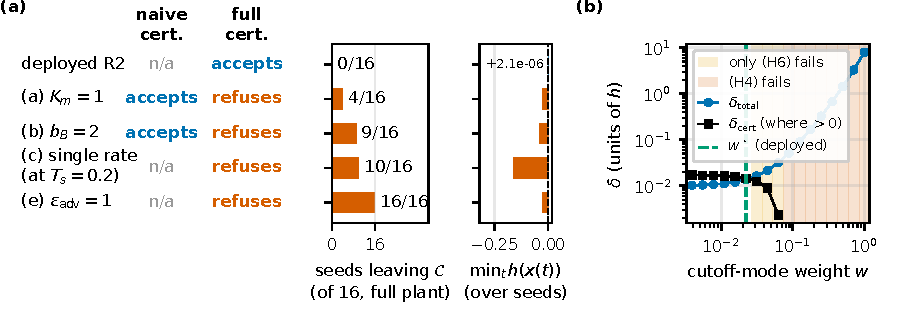
\includegraphics[width=\textwidth]{figures/main_fig_results.pdf}}
\end{figure}

\paragraph{Ablations.}
Each ablation alters one component at the deployed $w^\star$, and the full certificate refuses each (Figure~\ref{fig:results}(a)). Ablation (a) is a projection-based reduced-order certificate without a tail term, at $K_m = 1$: the naive certificate accepts, and 4 of 16 seeds leave the safe set. Ablation (b) is a 2-bit network certified as if it were its teacher: the naive certificate without the quantization term accepts, and 9 of 16 seeds leave the safe set. Ablation (c) holds a single command per period; at the deployed period it has $\dtot = 0.01702 > \dcert = 0.01456$ and is refused, while the multi-rate loop has $\dtot = 0.01356$, and none of its seeds leaves the safe set there within the horizon. At $T_s = 0.2$, where both loops are uncertified, the single-rate loop exits on 10 of 16 seeds; the multi-rate loop at that period is reported in the supplement. Ablation (e) raises the adversary to $\eadv = 1$: all 16 seeds exit, and at the largest certifiable level $\eadv^\star = 0.004223$ none does.


\paragraph{Refusals and the frontier.}
The certificate refuses 6 configurations: a look-up table indexed by $z$ instead of $v$, whose codesign window is empty, its lower end exceeding its upper end ($9,5$); $u_{\max}$ below the (H-sat) bound; unfiltered advection; the plain projector $w = 1$; the longer period $T_s = 5\times10^{-4}$, where $\dtot = 0.01821 > \dcert = 0.01455$; and all timing constants scaled by 10. Over 17 values of $w$ from 1 down to 0.003906, with the open loop unsafe at every value, the certificate accepts for $w \le 0.0221$ and refuses above it, through (H6) and then (H4) (Figure~\ref{fig:results}(b)). For the plain projector, on the scanned grid, the certified advection speeds ($c \le 0.02$, P\'eclet at most 0.4) and the open-loop-unstable ones ($c \ge 0.5$, P\'eclet at least 10) are disjoint. The frontier is set by the supremum over the $L^2$-type domain $\XO$ in $M_\perp$, which charges cutoff-mode advection at full strength. The deadzone result of Proposition~\ref{S-prop:deadzone_stability} holds in R1, where $\mu_R = 0.5$ exceeds the $P$-norm sector modulus $\Lsec = 0.1204$ of $F_{\mathrm{nl},r}$: the mid-tread deadzone silences the table late in the run, while the mid-rise quantizer of ablation (d) chatters at every tested $b_A$ (between 121.6 and 953.1 sign switches per unit time; Experiment 5 of the supplement); in R2, $\Lsec = 2.392 > \mu_R$ and it does not apply. Corollary~\ref{S-cor:stochastic_w2} is exercised in R1 at noise level $\sigma^\star = 0.007$: 0 of 2000 paths exit, the Clopper--Pearson upper limit 0.001843 lies below $\alpha = 0.05$, and the horizon bound $T_{\mathrm{TTL}} = 2022$ exceeds the horizon $T = 2$ by a factor 1011. The corollary is infeasible in R2 because the stochastic budget adds $\gamma_0\hact = 0.007237$ to $\dtot$, more than the margin $9.994\times10^{-4}$. ETD2RK step-halving ratios are 4.002 to 4.045. Every constant is computed in float64 from the operators, and the repository's 248 assertions and 65 tests regenerate every number.

% =====================================================================================================================
\section{Limitations and conclusion}
\label{sec:limits}

The certified plant is the lattice with filtered advection at $w^\star = 0.0221$; unfiltered advection and the plain projector are refused, and certifying full-strength cutoff-mode advection at the unstable P\'eclet numbers would need a different formulation, for example an $H^1$-bounded domain, whose effect on a smooth field the filter weight mimics heuristically (Remark~\ref{S-rem:rda_cutoff}); the theorem does not have one. The sampling period $T_s = 3\times10^{-4}$ is set by the certificate, not by the plant, which is sampled $1.714\times10^{4}$ times per slowest plant period in R2; the hold term is 0.4872 of $\dtot$, the price of a continuous-time guarantee with a Lipschitz hold bound (Section~\ref{sec:numerics}). On every certified run the minimum of $h$ is attained at the initial instant, and the dip floor $-\hdip$ is never reached. Theorem~\ref{thm:main_cbf} assumes exact acquisition of $z_k$ and exact latch instants; rounding of the Path-A input by $\varepsilon_z$ adds $\LTz\varepsilon_z$ to $\eA$ (Remark~\ref{S-rem:lut_variants}).

The stochastic extension is feasible in R1 only, its horizon bound is 1011 times the tested horizon, and every stochastic run uses $r_{W_2} = 0$. Proposition~\ref{S-prop:deadzone_stability} does not apply in R2 because $\Lsec > \mu_R$ there. The evidence is one benchmark class in two regimes. Ablations (a), (b) and (c) are paradigm-level baselines, not reimplementations of published methods; (b) is a 2-bit network and (c) has no naive verdict. Below $w^\star$ the single-rate budget closes (first at $w = 0.01562$), so $w^\star$ is the largest grid value at which every ablation is refused. Under the quadratic barrier, $\theta_{\mathrm{GS}} = 0$ (linear port feedback) maximises $\eta_{\mathcal{T}}$, so on this benchmark the neural teacher is not needed for authority; it is the object whose quantization and verification the budget must charge. A task on which a nonlinear neural policy beats linear port feedback on $\dcert$ is future work. The margin in R2 is $\dcert - \dtot = 9.994\times10^{-4}$.

Each of the six gaps between the verified model and the running plant costs one term of \eqref{eq:budget}, and Theorem~\ref{thm:main_cbf} turns a closed budget into full-order safety for all time; on the lattice the budget closes at utilisation 0.931 and names the hold term as the one to sharpen. The budget is the certificate, and its refusals are results.

\subsection*{Generative AI Use}
Generative AI tools assisted with drafting and editing the text, writing and testing the code, and checking derivations and references. The authors reviewed all theorems, proofs, experiments and claims and take full responsibility for the content.

\acks{Acknowledgments to be added.}

\bibliography{references}

\end{document}
